\documentclass[12pt,a4paper]{report}
\usepackage[utf8]{inputenc}
\usepackage[french]{babel}
\usepackage[T1]{fontenc}
\usepackage{amsmath}
\usepackage{amsfonts}
\usepackage{amssymb} 
\usepackage{mathtools}
\usepackage{xcolor}
\usepackage{graphicx}
\usepackage[left=2cm,right=2cm,top=2cm,bottom=2cm]{geometry}
\begin{document}



\begin{center}
	\textbf{Première Partie: Notion sur les éléments du thème}
\end{center}



\begin{center}
\textbf{I-Notion de caméras}	
\end{center}

Selon la Ref. \cite{noauthor_quest-ce_nodate} une caméra est un dispositif qui capture la lumière et la transforme en image. Elle le fait à travers une lentille, qui concentre la lumière sur une surface sensible à la lumière, où une image se forme. \\
Il ya deux catégories de caméras :
\begin{itemize}
	\item \textbf{Les caméras numériques}: Elles capturent des images par voie électronique à l’aide d’un capteur.
	\item\textbf{les caméras à pellicule}: Elles utilisent une bande de pellicule enduit de produits chimiques photosensibles. Elles sont utilisées pour la réalisation de film.\\
	La pellicule est une feuille mince formant le support souple à une couche sensible , elle définit chaque détaille d'une photo(couleurs, contrastes, exposition, grain, etc)\\
\end{itemize}

 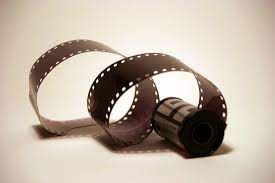
\includegraphics[scale=1]{image/pellicule.jpeg}
 
      image d'une pellicule\\
      
   \textbf{1. Les parties essentiels d'une caméra\\}
   
Les parties essentielles d’une caméra comprennent : \\
\begin{itemize}
\item \textbf{Le corps :} Il tient toutes les composantes ensemble. \\
\item \textbf{La lentille :} Elle met la lumière au centre du capteur d’image. \\
\item \textbf{L’obturateur :} Il contrôle la quantité de lumière qui atteint le capteur.\\ 
\item \textbf{L’ouverture :} Elle contrôle la quantité de lumière que l’objectif laisse entrer.Sa taille est mesurée en f-stops. Un plus petit nombre de f-stop indique une plus grande ouverture (plus de lumière) et un nombre de f-stop plus grand indique une plus petite ouverture (moins de lumière).\\
\item \textbf{Le capteur d'image:} IL convertit le rayonnement électromagnétique en un signal électrique analogique. Ce signal est ensuite amplifié, puis numérisé par un convertisseur analogique-numérique et enfin traité pour obtenir une image numérique. La taille du capteur de caméra a un impact significatif sur la qualité de l’image.En effet des capteurs plus grands permettent d'avoir généralement une meilleure qualité d’image, surtout dans des conditions d’éclairage faible. Ils ont également une plus grande surface pour la prise de détails, ce qui peut se traduire par des photos plus nettes et plus détaillées.\\
\end{itemize}

\textbf{2.Le micrologiciel d'une caméra \\}

Le micrologiciel ou firmware d'une caméra est un type de logiciel programmé dans le matériel de la caméra, il contrôle toutes les fonctions de la caméra,de la mise au point automatique et des paramètres d’exposition jusqu’au traitement et au stockage des images.\\

\textbf{3.Les différents types de caméras \\}

D'après la Ref. \cite{noauthor_les_2015} ils existes sept types de caméras qui sont entre autre :\\

\begin{itemize}
	\item \textbf{Les caméras de smartphones} : Ce sont les caméras intégrés dans les téléphones portables.De nos jours la qualité des images qu'ils produisent les amènes à rivaliser avec les caméras professionnels qui existe sur le marché.Elles sont utilisés pour les web vidéos, clips, interviews, courts-métrages, etc......\\
	
	\item \textbf{Les Camescopes} sont des caméras utilisé par le grand public pour leurs souvenir de famille.Aujord'hui elles sont rare sur le marché car ils sont remplacé par les smartphones.seuls les plus chers parviennent à se démarquer par leur qualité d’image . Ils sont souvent de petite taille, élaborées pour automatiser la plupart des réglages et disposent bien souvent de petits capteurs mais jamais d’entrées audio.\\
	
	\textbf{Exemple :\\}
	\begin{itemize}
		\item \textbf{Canon Vixia HF R52} dispose d'un capteur d'image CMOS Full HD de 3,28 mégapixels, un processeur d'image DIGIC DV 4 capturant des vidéos Full HD 1920 x 1080 ,une clé USB interne de 32 Go,un Wi-Fi et un écran LCD 3 pouces. \\
		\item \textbf{Sony HDR PJ275} dispose d'une clé USB de 8 Go avec un projecteur intégré de Sony capture des vidéos Full HD 1920 x 1080 à 60p et des images fixes de 9,2 MP. Il est doté d'un capteur CMOS Exmor R 1/5,8" et d'un objectif zoom grand angle Carl Zeiss Vario-Tessar avec zoom optique 27x plus zoom numérique Clear Image 54x.\\
		
		\item \textbf{Panasonic HC W850} dispose d'un format AVCHD, un Capteur BSI 1/4 pouce, une Zoom de 20 x , une distance focale en 24x36 	de 29,5-612 mm , une stabilisation d'image et une dimensions 	65 x 73 x 139 mm. \\		 
	\end{itemize}
		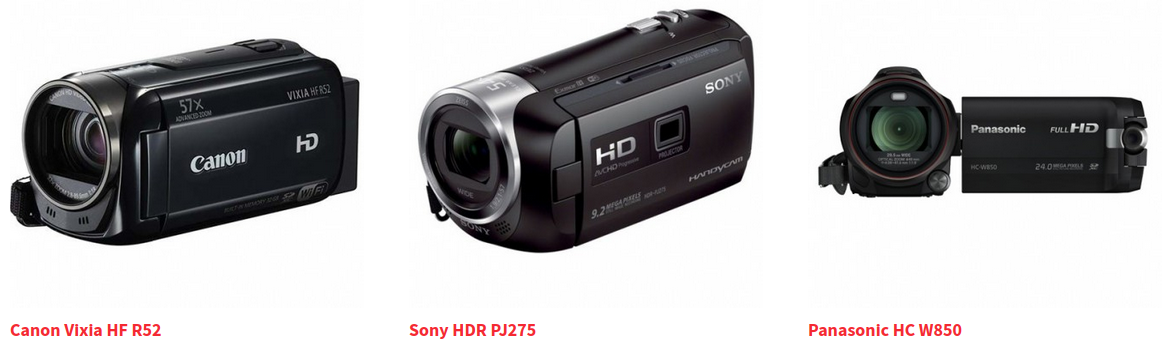
\includegraphics[scale=0.38]{image/camescopes.png} \\
		
	\item \textbf{Les DSLR(digital single-lens reflex)} sont des appareils photo réflex numériques disposant d’une fonction de capture vidéo.Ils sont caractérisés par la taille de leur capteur qui permettent d'avoir des images de qualités, d’objectifs interchangeables qui permettent de varier les rendus stylistiques en jouant avec les différents types de « cailloux » selon les photographes et la petite taille des lentilles (comparé à ceux d’une caméra pro) rend accessible le prix des objectifs.\\
	
	\textbf{Exemple :\\}
	
	\begin{itemize}
		\item \textbf{Canon 5D Mark III} dispose d'un Capteur plein format de 22,3 mégapixels , un collimateurs AF 61 , une prise de vue en continu à 6 ips, une sensibilité de 100 à 25 600 ISO, extensible à 102 400 ISO, une vidéo Full HD avec contrôle manuel,une sortie HDMI non compressée en Full HD 8 bits 4.2.2, un processeur DIGIC 5+ 14 bits, une étanchéité aux intempéries, un écran de 8,11 cm (3,2 pouces) avec 1 040 000 points. \\
		\item \textbf{Nikon D800} dispose d'un capteur CMOS au format FX (24 x 36) de 36,3 millions de pixels , une sensibilité de 100 à 6400 ISO, un moniteur ACL de 8 cm (3,2 pouces), une connexion au réseau sans fil et Etherne ,.\\
		
		\item \textbf{Canon 7D} dispose d'une résolution d'image maximale de la webcam, Vitesse d'obturation maximale 30 - 1/8000. \\		 
	\end{itemize}
	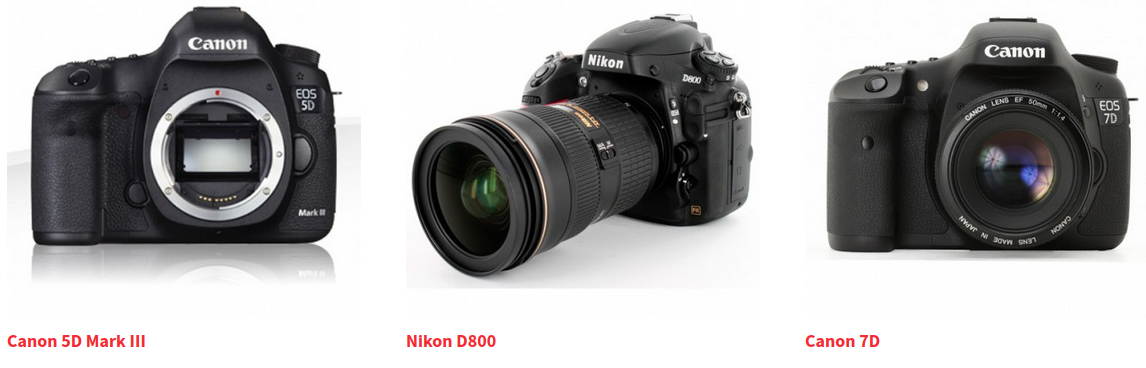
\includegraphics[scale=0.38]{image/DSLR.png} \\
	
\item \textbf{Les Caméras dites « Prosommateurs »} Le mot « prosommateur » est composé de « pro » issu de production et « sommateur » de consommateur. On appelle les prosommateurs les personnes qui achètent des produits avec une certaine exigence car ils ont pour intention d’utiliser un produit dans un cadre de production.Ces caméras assez récentes sont venues perturber la frontière entre camescopes et caméras professionnelles en insérerant une gamme intermédiaire répondant aux besoins des petits producteurs indépendants.Elles sont généralement d’une taille supérieure à un camescope mais bien moins encombrante que les caméras pro de plateau ou de cinéma et proposent une excellente qualité d’image.


\textbf{Exemple :\\}

\begin{itemize}
	\item \textbf{Sony PMW 300}renferme trois capteurs CMOS Full HD Exmor 1/2 pouce et conserve le codec MPEG-2 Long GOP échantillonné en 4:2:2 sur un débit HD de 50 Mbit/s. . \\
	
	\item \textbf{Panasonic AG HPX250} dispose d'un Batterie autonomie réelle (ou continue)NC,d'un Capteur 3 x 2millions de pixels,d'une carte mémoire (P2), d'une compression MPEG-4 DV, d'un diamètre filetage 72 mm , d'une dimensions
	180 x 195 x 438 mm.\\
	
	\item \textbf{Canon XF 205} dispose d'un objectif à grand-angle 20× f/1,8 garantissant d'incroyables prises de vues à grande distance,d'un capteur HD CMOS Pro offrant une qualité d'image exceptionnelle, même en basse lumière etc...\\		 
\end{itemize}
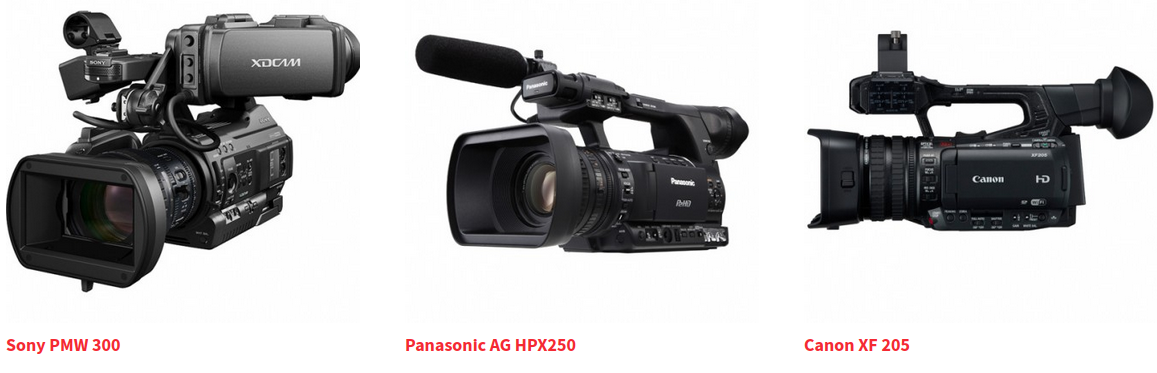
\includegraphics[scale=0.38]{image/prosommateur.png} \\


\item \textbf{Caméras Professionnelles} Les caméras professionnelles sont de très grosses caméras disposant des capteurs les plus gros, les objectifs y sont évidemment interchangeables,le paramétrage de la colorimétrie y est bien souvent plus poussé, et elle sont systématiquement synchronisable par timecode. 

\textbf{Exemple :\\}

\begin{itemize}
	\item \textbf{Panavision Panaflex Millenium}\\
	
	\item \textbf{Arri Arriflex D-21}\\
	
	\item \textbf{Aaton Penelope}\\		 
\end{itemize}
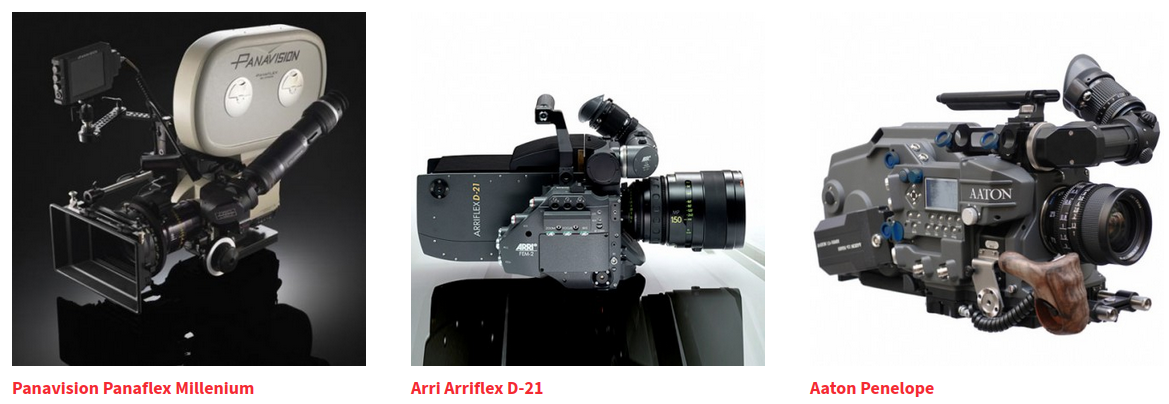
\includegraphics[scale=0.38]{image/professionnel.png} \\

\item \textbf{Les Caméras de type "Super Concentré"} « Super Concentré » est un terme inventer selon la Ref. \cite{noauthor_les_2015} pour catégoriser cette dernière tendance d’appareils. Ce qui les qualifie c’est avant tout de très grands capteurs supérieurs à la majorité des caméras prosommateurs qui leur confère une qualité d’image cinématographique comparable aux caméras professionnelles. Les objectifs sont interchangeables, et sont capables d’exporter les rushs au format RAW qui permet une grande souplesse d’ajustement en post-prod. 
	
	\textbf{Exemple :\\}
	
	\begin{itemize}
		\item \textbf{Camera Red} \\
		
		\item \textbf{Camera Blackmagic} \\
		
		\item \textbf{Canon C300}\\		 
	\end{itemize}
	\includegraphics[scale=0.38]{image/super consentré.png} \\
	
\item \textbf{Les Caméras dédiées} sont des caméras qui sont particulièrement dédiées à un besoin spécifique comme les caméras miniatures pour les sports extremes ou l’embarcation dans les véhicules motorisés, les caméras à haute cadence pour le slow motion, les caméras 3D, ou encore les caméras drones.
	
	
	\textbf{Exemple :\\}
	
	\begin{itemize}
		\item \textbf{Go Pro}\\
		
		\item \textbf{Quadrirotor DJL Phantom 2 Vision}\\
		
		\item \textbf{Panasonic AG 3DA1}\\		 
	\end{itemize}
	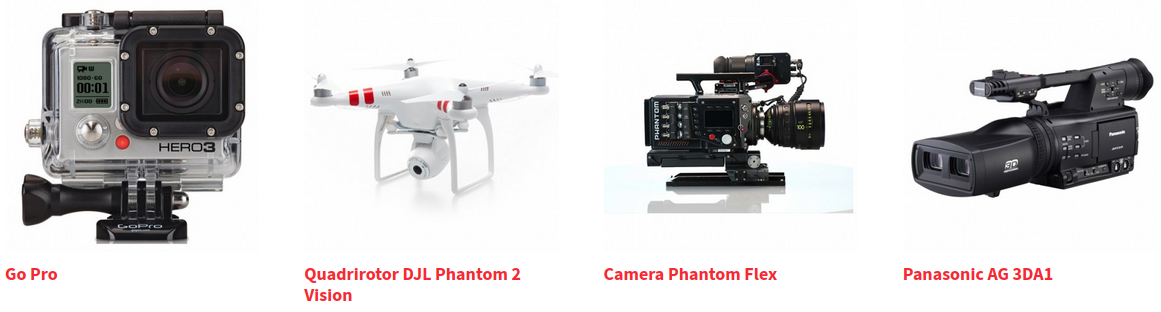
\includegraphics[scale=0.38]{image/caméras dedié.png} \\	
\end{itemize}









%notion de calibrage 
\newpage

\begin{center}
	\textbf{II-Notion de calibrage}	\textcolor{red}{Toute cette parte est à modifié}
\end{center}


D'après la Ref.\cite{orteu_calibrage_nodate} le calibrage d'une caméra consiste à déterminer la relation mathématique existant entre les coordonnées des points 3D de la scène observée et les coordonnées 2D de leur projection dans l'image (points-image).\\
Alors calibrer une caméra consiste à estimer sa fonction de transfert.\\

\textit{schémas d'illustration\\}

\includegraphics[scale=0.5]{image/illustration caméras.png} \\
 \textcolor{red}{fin de la partie}\\

   \textcolor{red}{Toute cette parte est à revoir pour bien mettre dans la notion de calibrage}\\
   
L'étalonnage de la caméra est une étape nécessaire en vision par ordinateur 3D afin d'extraire des informations métriques à partir d'images 2D. De nombreux travaux ont été réalisés, à commencer par la communauté de la photogrammétrie (voir [2, 4] pour n'en citer que quelques-uns), et plus récemment en vision par ordinateur ( [9, 8, 20, 7, 23, 21, 15, 6, 19] pour n'en citer que quelques-uns). Nous pouvons classer ces techniques grossièrement en deux catégories : \\
Calibrage photogrammétrique. L'étalonnage est effectué en observant un objet d'étalonnage dont la géométrie dans l'espace 3D est connue avec une très bonne précision. L'étalonnage peut être effectué de manière très efficace [5]. L'objet d'étalonnage est généralement constitué de deux ou trois plans orthogonaux entre eux. Parfois, un plan subissant une translation précisément connue est également utilisé [20]. Ces approches nécessitent un appareil d'étalonnage coûteux et une configuration élaborée.\\
Auto-calibrage. Les techniques de cette catégorie n’utilisent aucun objet d’étalonnage. En déplaçant simplement une caméra dans une scène statique, la rigidité de la scène fournit en général deux contraintes [15] sur les paramètres internes des caméras à partir d'un déplacement de caméra en utilisant uniquement les informations d'image. Par conséquent, si les images sont prises par la même caméra avec paramètres internes fixes, les correspondances entre trois images suffisent pour récupérer à la fois les paramètres internes et externes qui permettent de reconstruire la structure 3D jusqu'à une similarité [14, 12]. Bien que cette approche soit très flexible, elle n’est pas encore mature [1]. Comme il existe de nombreux paramètres à estimer, nous ne pouvons pas toujours obtenir des résultats fiables.\\
 \textcolor{red}{fin de la partie}\\
 


\begin{center}
\textbf{A- Modèles de caméras} \textcolor{red}{Toute cette parte est à mettre dans une autre partie}
\end{center}

Ref.\cite{orteu_calibrage_nodate} décrit les principaux modèles de caméra utilisés ainsi que les principales méthodes proposées pour déterminer les paramètres du modèle choisi car selon lui calibrer une caméra, c'est choisir un modèle de caméra a priori et déterminer ensuite les paramètres de ce modèle.\\

\begin{center}
 \textbf{a.Le modèle sténopé } 	
\end{center}

	 
 Le modèle sténopé est décrit par 5 paramètres intrinsèques  $ (Cx \ Cy \ fx \ fy \ 0) $ et 6 paramètres extrinsèques (3 pour la rotation et 3 pour la translation). \\
Le modèle sténopé modélise une caméra idéale (simple projection perspective) et ne prend pas en compte les éventuelles distorsions géométriques induites par le système optique utilisé alors que , pour obtenir des mesures dimensionnelles précises, il est indispensable de prendre en compte les distorsions géométriques induites par le système optique utilisé.\\

\begin{center}
	\textbf{b.Le modèle sténopé avec prise en compte des distorsions} 	
\end{center}

\begin{itemize}
	\item \textbf{Approche paramétrique (classique)} 
L'approche paramétrique classique consiste à modéliser la distorsion en enrichissant le modèle sténopé par
des termes supplémentaires (le modèle devient alors non linéaire). Dans cette approche, le modèle s'inspire de
la théorie des aberrations géométriques des systèmes centrés en rajoutant des termes correctifs
correspondants à différents types de distorsions : distorsion radiale, prismatique, de décentrage\\

\item \textbf{Approche non-paramétrique}
Ils s'agit d'une modélisation purement mathématique (approche type « boîte noire ») visant à
déterminer la fonction de distorsion qui traduit au mieux la façon dont l'image idéale est distordue.\\
\end{itemize}
 \textcolor{red}{Fin}\\

\begin{center}
	\textbf{B- Les méthodes de calibrages} \textcolor{red}{Toute cette parte est à revoir}
\end{center}


Selon la Ref.\cite{remondino_digital_2006} il existe deux approches sur l'étalonnage d'une caméra dont 
l'étalonnage des caméras en photogrammétrie qui donne une reconstruction précise d'un modèle 3D à partir d'images 2D et l'étalonnage en vision par ordinateur qui donne une interprétation et une compréhension du contenu d'images et de vidéos. \\
Dans de nombreuses applications, notamment en vision par ordinateur (CV), seule la distance focale est récupérée alors que pour des mesures photogrammétriques précises, tous les paramètres d'étalonnage sont généralement utilisés.\\
Les algorithmes proposés sont généralement basés sur des modèles de caméras prospectives ou projectives.



\begin{center}
	\textbf{ a. Etalonnage photogrammétrique}
\end{center}

\begin{itemize}
	\item Dans la Ref.\cite{orteu_calibrage_nodate} Une méthode a été décrite par \textbf{JEAN-JOSÉ ORTEU} qui selon lui est la méthode considérée aujourd'hui comme la plus performante . Cette méthode consiste à acquérir n images d'une mire (plane) composée de p points déplacée librement(rotations et translations) dans le champ de vue de la caméra. La méthode de calibrage décrite est dite de type photogrammétrique. Elle permet d'estimer en même temps tous les paramètres du modèle de caméra ainsi que les points tridimensionnels de la mire. Par conséquent, la géométrie de la mire de calibrage n'a pas besoin d'être connue avec précision a priori.\\
	
	\item Un modèle de caméra \cite{remondino_digital_2006}basé sur la projection en perspective, où l'implication est que
	l'IO est stable (au moins pour un réglage de distance focale donné) et que tous les écarts par rapport à la colinéarité, linéaires et non linéaires, peuvent être pris
	en compte. Ce modèle basé sur une équation de colinéarité nécessite
	généralement cinq correspondances de points ou plus au sein d'un réseau multi-images et, en raison de sa nature non linéaire, nécessite des approximations des valeurs de paramètres pour l'ajustement du paquet des moindres carrés dans lequel les paramètres d'étalonnage sont récupérés.\\
	
	\item Un modèle de caméra projective prenant en charge la projection plutôt que la reconstitution de scène euclidienne. Un tel modèle, caractérisé
	par les modèles de matrice essentielle et de matrice fondamentale, peuvent s'adapter à des distances focales variables et inconnues, mais nécessite un minimum de 6 à 8 correspondances de points pour faciliter une
	solution linéaire, qui est invariablement assez instable. Non-perturbations des coordonnées d'image linéaires telles que la distorsion de l'objectif ne sont pas faciles à traiter dans de tels modèles.\\
\end{itemize}

\begin{center}
	\textbf{b. Etalonnage en vision par ordinateur}
\end{center}

Notre compréhension sur l'étalonnage de la caméra en vision par ordinateur se base sur la littérature de la Ref. \cite{remondino_digital_2006}. Selon lui les modèles d'étalonnage pour la vision industrielle et par ordinateur utilisent traditionnellement des grilles de référence, la matrice d'étalonnage K étant déterminé à l'aide d'images d'un réseau de points d'objets connu (par exemple un motif en damier). Les méthodes couramment adoptées sont celles de Tsai (1987),Heikkila et Silven (1997) et Zhang (2000) Cité dans celui-ci. Ceux­ci sont tous basés sur le modèle de caméra sténopé et incluent des termes pour modéliser la distorsion radiale.\\

Aussi, dans la vision par ordinateur on peut avoir l'auto-étalonnage Ce terme en CV est utilisé lorsqu'aucun objet d'étalonnage n'est utilisé et que les propriétés métriques de la caméra et de la scène imagée sont récupérées à partir d’un ensemble d’images « non calibrées », en utilisant des contraintes sur les paramètres de la caméra ou sur la scène imagée. L'auto-étalonnage est généralement adopté dans la modélisation 3D pour mettre à niveau une reconstruction projective vers une reconstruction métrique(c'est-à-dire déterminée jusqu'à une transformation euclidienne arbitraire et un facteur d'échelle).\\


Dans l'article \cite{adil_novel_2022} dont le titre signifie \textit{un nouvel algorithme pour la mesure des distances à l'aide d'une camera stéréo} relate la manière de calculer la distance entre un objet et une caméra stéréo(une caméra stéréo permet de capturer des images en 3D en utilisant deux objectifs pour obtenir une perception de la profondeur similaire à celle de la vision humaine.) en utilisant la bibliothèque de opencv avec python . Pour cela deux caméras similaires ont ­été utilisées pour réaliser les expériences en temps réel. Les résultats ont montré que l'algorithme calcule la distance(190cm maximum) avec un taux de 5 pour cent avec un temps moyen de traitement de 0.355s . \\


Le calibrage de la caméra pour le calcul des distances de saut en longueur a été plus abordé dans l'article \cite{jin_2022-3-exploring_2022} où l'auteur a réalisé un système de mesure de distance pour le saut en longueur à l'aide de la vision par ordinateur et l'intelligence artificiel.Il a utilisé Opencv pour le calibrage, la correction de la distorsion de la caméra et l'extraction des contours des images. Ensuite il a utilisé Openpose pour la détection de la posture humaine et enfin il a utilisé l'algorithme de transformation de perspective géométrique pour le calcul de la distance.

 \textcolor{red}{Fin de la partie}\\




\newpage                        

\begin{center}
	\textbf{Deuxième Partie: Début des tests}
\end{center}


 Ces tests seront basés sur les méthodes de télémétrie , l'application de  l'intelligence artificiel, et la vision par ordinateur.
 \begin{center}
 	\textbf{Définition des différents thermes}
 \end{center}

\begin{itemize}
	\item La télémétrie: est un processus de mesure à distance où des données sont collectées à partir de dispositifs éloignés, puis transmises à un emplacement central pour analyse ou surveillance.\\
	
	\item L'intelligence artificiel: est un domaine de l'informatique qui se concentre sur la création de systèmes informatiques capables d'accomplir des tâches qui nécessiteraient normalement une intelligence humaine.\\
	
	\item La vision par ordinateur: concerne le développement de systèmes qui peuvent « voir » et interpréter les images et les vidéos de manière similaire à la vision humaine.
\end{itemize}


\begin{center}
	\textbf{1.Calibrage et correction de la distorsion du caméra}
\end{center}

L'étalonnage de la caméra est une étape nécessaire en vision par ordinateur 3D afin d'extraire des informations métriques à partir d'images 2D.\\

Opencv traite les caméras avec un modèle sténopé (Le modèle sténopé est une représentation mathématique d'un objet 3D projeté dans un espace 2D )\\

Le calibrage est utilisé pour obtenir les paramètres suivants:
\begin{itemize}
	\item Les paramètres internes appelé paramètres intrinsèques composé de :
	\begin{itemize}
		\item distance focal(fx, fy)
		\item les points principales (cx et cy)
		\item les distorsions (k1,k2,p1,p2,k3)
	\end{itemize}
	\item Les paramètres externes appelé paramètres extrinsèques :
		\begin{itemize}
		\item Rotation(R)
		\item Translation(T)
	\end{itemize}
	
\end{itemize}



\begin{center}
	\textbf{Résumé de la méthode de Zhang Zhengyou \cite{zhengyou_zhang_flexible_1999}}\textcolor{red}{Plusieurs notions doivent être ajouté pour la description de la méthode}\\
\end{center}

La méthode de calibrage proposé par zhang Zhengyou connue sous le nom méthode de calibrage de caméra basée sur le plan d'échiquier est une technique simple, flexible et réalisable à moindre coût.\\ 
Cette technique proposée nécessite uniquement que la caméra observe un motif plan affiché dans quelques (au moins deux) orientations
différentes. Le motif peut être imprimé et fixé sur une surface plane « raisonnable » (par exemple, une couverture de livre rigide).La caméra ou le motif planaire peuvent être déplacés à la main. L'approche proposée se situe entre le calibrage photogrammétrique et l'auto-calibrage car ils utilisent des informations métriques 2D plutôt que 3D ou purement implicites. Dans l'article le travail a été regroupé en quatre sections qui sont: 
\begin{itemize}
	\item \textbf{Les contraintes de bases liées à l'observation d'un seul plan:} Comporte la notation de la matrice du caméras et les deux contraintes lié aux paramètres intrinsèques.\\
	
	\item \textbf{La procédure de calibrage:}  aborde d'abord la solution fermé qui permet de résoudre les contraintes liées aux paramètres intrinsèques , ensuite la technique d'optimisation non linéaire basée sur le critère du maximum de vraisemblance pour affiner les paramètres avec l'algorithme de Levenberg ­Marquardt et enfin la prise en compte de la distorsion radial de la lentille pour corriger la distorsion.\\
	
	\item \textbf{La section 4} étudie les configurations dans lesquelles la technique d'étalonnage proposée échoue\\
	
	\item \textbf{La section 5} fournie les résultats expérimentaux.
	 
	 
\end{itemize}



\begin{center}
	\textbf{Etude de la methode de zhang}
\end{center}

L'objectif principal de l'étalonnage de la caméra est de déterminer les propriétés intrinsèques inconnues de la caméra, c'est-à-dire les éléments de la matrice A.\textcolor{red}{à mettre après la notation}

\begin{center}
	\textbf{Mise en oeuvre de la méthode}\textcolor{red}{À bien structuré après}
\end{center}
	
	
\begin{center}
	\textbf{I.Utilisation de la caméra}
\end{center}

La caméra mis à notre disposition est un Hercule HD Twist et nous allons voir comment l'accéder en utisant python et opencv.


\begin{center}
	\textbf{II.Implémentation de l'algorithme}
\end{center}

L'impléméntation de la methode de Zhang Zhengyou va se basé sur les algorithmes de Wilhelm Burger cité dans son document \cite{burger_zhangs_2016} .\\

\textcolor{red}{Mettre un algorithme ici \\}

\textbf{Explication:}Cet algorithme est une vue d'ensemble de l'algorithme de calibrage de caméra de Zhang. il présente une fonction \textbf{Calibrate} qui prend en entrée une séquence ordonnée de points 3D sur la cible planaire (X) et une séquence de vues, où chaque vue est une séquence ordonnée de points d'image observés (U˙). Elle retourne les paramètres intrinsèques estimés de la caméra (matrice de caméra A) et les paramètres de distorsion (k), ainsi que les transformations extrinsèques (W) pour chaque vue. 










































\newpage

\begin{center}
	\textbf{A.Installation des dépendances}
\end{center}

\textbf{Installation d'opencv sur Window}

\begin{itemize}
	
	\item Installation de python : Se rendre sur le site https://www.python.org/downloads/ et télécharger la dernière version. Contrairement à ubuntu pip est en même temps lors de l'installation de python. Nous avons installé la version 3.12.2 pour python et 24.0 pour PIP\\
	
	\item Installation de Opencv: Taper \textbf{PIP install opencv-python} pour l'installation, Numpy est aussi installer. nous avons la version 4.9.0 pour Opencv et 1.26.4 pour Numpy.
	
	\item Installation de matplotlib: Tapez \textbf{pip install matplotlib} pour l'installation de la dernière version. nous avons installer la version 3.8.3
	
	\item Installation d'anaconda: Nous avons installer anaconda pour pouvoir utilisé l'application web Jupyter Notebook.\\
	   
\end{itemize}


\begin{center}
\textbf{Installation des dépendances}	
\end{center}


\textcolor{red}{Intallation d'Opencv et python a recupéré dans le fichier note}\\

\textbf{Installation de Matplotlib \\}

Taper \textbf{pip3 install matplotlib} \\

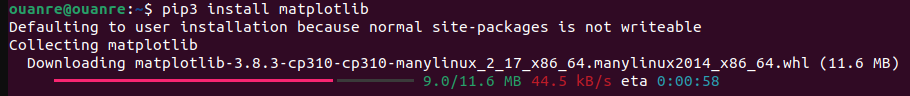
\includegraphics[scale=0.5]{image/instalation de matplotlib1.png} \\

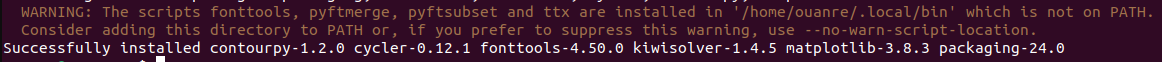
\includegraphics[scale=0.40]{image/installation de matplotlib2.png}\\

\textbf{Installation de Numpy}




 

















\newpage
\bibliographystyle{smfplain}
\bibliography{mybiblio}
\end{document}